% Chapter 8
\section{Radial Basis Function Networks (RBFNs)}\label{chap:rbf}

Building on the multilayer perceptron (MLP) architecture (\Cref{chap:mlp}) and its training machinery (\Cref{chap:backprop}), this chapter introduces radial basis function networks (RBFNs): three\hyp{}layer models with fixed nonlinear bases and a linear readout. \Cref{fig:roadmap} places this as the kernel/prototype branch alongside the MLP path.

\begin{tcolorbox}[summarybox, title={Learning Outcomes}]
\begin{itemize}
    \item Explain the architecture and training stages of RBF networks (center selection, width tuning, linear solve).
    \item Relate RBF solutions to linear estimators (normal equations, pseudoinverse, Wiener filtering) and know when ridge regularization is needed.
    \item Compare RBFNs to kernelized methods and other nonlinear classifiers to choose appropriate models in practice.
\end{itemize}
\end{tcolorbox}

\begin{tcolorbox}[summarybox, title={Design motif}]
Make the nonlinearity explicit: use a fixed (or lightly tuned) basis expansion in the hidden layer, then learn the output weights with linear-algebra tools.
\end{tcolorbox}

\subsection{Overview and Motivation}
\label{sec:rbf_overview_and_motivation}

\paragraph{How to read this chapter.}
We start with the three-layer picture and the basis-function intuition, then write the model in matrix form and show how training becomes a regularized least-squares solve. Near the end we connect the finite-basis view to the kernel viewpoint. The Wiener-filter box is optional context if you want the signal-processing parallel.

Unlike MLPs, which learn weights in every layer, an RBFN separates the job into two parts. The hidden layer provides a fixed nonlinear feature map (set by centers and widths). The output layer then learns a linear combination of those features. That split is the main story in this chapter: choose the basis, then solve for the readout.

The key idea is that ``nonlinear'' can come from the representation rather than the readout. Radial basis functions act like localized, kernel-style features; once you lift inputs into that feature space, the output layer is still linear, and the weights are responsible for finding the separating border. This is closely related to the kernel trick used in SVMs; \Cref{app:kernels} collects the classical kernel viewpoint.

\Cref{chap:supervised} frames this as a bias--variance tuning problem (choose capacity, regularization, and diagnostics via learning curves). Kernel methods such as kernel ridge regression and SVMs interpret the same trade-off through an RBF kernel matrix; here we keep the bases explicit, then connect to the dual/kernel view later in the chapter.

\paragraph{Running example: XOR as a representation problem.}
XOR is the smallest reminder that a single line in the input space is not always enough. The point of RBF networks is not that the output layer becomes complicated; it stays linear. The complication is pushed into the feature map: the hidden units apply localized, kernel-like transforms, and the output weights are responsible for finding the separating border in that transformed space. We will return to XOR twice: first to see the feature map, then to see how the linear solve chooses the readout weights.

\paragraph{Centers from clustering (a practical default).}
The hidden layer of an RBF network is easiest to understand when its centers are viewed as K-means prototypes: pick a coverage of the input space that reflects the data distribution, assign widths accordingly, and let the output layer learn the linear weights on top of those prototypes. Unsupervised clustering up front makes the later supervised solve far more stable.

\subsection{Architecture of RBFNs}
\label{sec:rbf_architecture_of_rbfns}

The RBFN consists of three layers:

\begin{tcolorbox}[summarybox, title={Notation and shapes}]
We denote each basis response by \(\varphi_i(\mathbf{x})\); stacking them yields \(\mathbf{G}(\mathbf{x})\in\mathbb{R}^M\) with entries \(G_i(\mathbf{x})=\varphi_i(\mathbf{x})\). For a dataset of \(N\) samples, the corresponding design matrix \(\boldsymbol{\Phi}\in\mathbb{R}^{N\times M}\) stacks one transformed sample per row, with entries \(\boldsymbol{\Phi}_{ji}=\varphi_i(\mathbf{x}_j)=G_i(\mathbf{x}_j)\). This matches the design-matrix convention used in \Cref{chap:supervised}.
\end{tcolorbox}


\begin{figure}[t]
    \centering
    \begin{tikzpicture}[>=stealth, node distance=1.6cm]
        \tikzset{
            inputnode/.style={circle, draw, fill=gray!10, minimum size=0.8cm},
            rbf/.style={circle, draw, fill=cbBlue!15, minimum size=1cm},
            outputnode/.style={circle, draw, fill=cbOrange!20, minimum size=0.9cm}
        }
        % inputs
        \node[inputnode] (x1) {$x_1$};
        \node[inputnode, below=0.8cm of x1] (x2) {$x_2$};
        \node[below=0.6cm of x2] (dots) {$\vdots$};
        \node[inputnode, below=0.6cm of dots] (xd) {$x_d$};
        % rbf layer
        \node[rbf, right=2.0cm of x1] (h1) {$\varphi_1$};
        \node[rbf, right=2.0cm of x2] (h2) {$\varphi_2$};
        \node[right=2.0cm of dots] (dots2) {$\vdots$};
        \node[rbf, right=2.0cm of xd] (hm) {$\varphi_M$};
        % output
        \node[outputnode, right=2.5cm of h2] (y) {$\hat{y}$};
        % connections input to rbf
        \draw[->, gray!70] (x1) -- (h1);
        \draw[->, gray!70] (x1) -- (h2);
        \draw[->, gray!70] (x2) -- (h1);
        \draw[->, gray!70] (x2) -- (h2);
        \draw[->, gray!70] (xd) -- (hm);
        % rbf to output
        \draw[->, thick, cbOrange] (h1) -- node[above, sloped, font=\scriptsize] {$w_1$} (y);
        \draw[->, thick, cbOrange] (h2) -- node[above, sloped, font=\scriptsize] {$w_2$} (y);
        \draw[->, thick, cbOrange] (hm) -- node[below, sloped, font=\scriptsize] {$w_M$} (y);
        % bias
        \node[below=1cm of y, font=\scriptsize] (bias) {bias $b$};
        \draw[->, cbOrange, dashed] (bias) -- (y);
        % notes
        \node[align=left, font=\scriptsize, above=0.2cm of h1] {Centers/widths\\\((\boldsymbol{\mu}_i,\sigma_i)\) set by\\k-means or heuristics};
        \node[align=left, font=\scriptsize, right=0.3cm of y] {Linear weights \(w_i\)\\learned from data};
    \end{tikzpicture}
    % Avoid inline math in captions; it wraps poorly in some EPUB renderers.
\caption{RBFN architecture. Inputs feed fixed radial units parameterized by centers and widths; a linear readout with weights and bias is trained by a regression or classification loss. Only the output weights are typically learned, while centers and widths come from clustering or spacing heuristics.}
    \label{fig:rbf_architecture_weights}
\end{figure}
\FloatBarrier

\Cref{fig:rbf_architecture_weights} highlights the split between fixed radial features and a trained linear readout.

\paragraph{A picture to keep in mind}
Once you have the architecture in mind, it helps to visualize what the hidden layer \emph{does}. In one dimension, you can literally draw the bases as overlapping Gaussian bumps; the model output is a weighted sum of those bumps. \Cref{fig:rbf_gaussian_bumps} is the mental model we will reuse as we introduce centers, widths, and the final linear solve.

\begin{figure}[t]
    \centering
    \begin{tikzpicture}
        \begin{axis}[
            width=0.68\linewidth,
            height=0.34\linewidth,
            xlabel={$x$},
            ylabel={Activation},
            xmin=-4, xmax=4,
            ymin=-0.2, ymax=1.4,
            legend style={at={(0.02,0.98)}, anchor=north west}
        ]
            \addplot[cbBlue, dashed, mark=*, mark repeat=25, mark options={fill=cbBlue}, domain=-4:4, samples=200]{exp(-((x+2)^2))};
            \addlegendentry{$\varphi_1$}
            \addplot[cbOrange, dashed, mark=square*, mark repeat=25, mark options={fill=cbOrange}, domain=-4:4, samples=200]{0.8*exp(-((x-0.5)^2)/0.5)};
            \addlegendentry{$\varphi_2$}
            \addplot[cbGreen, dashed, mark=triangle*, mark repeat=25, mark options={fill=cbGreen}, domain=-4:4, samples=200]{0.9*exp(-((x-2.2)^2)/0.7)};
            \addlegendentry{$\varphi_3$}
            \addplot[cbPink, thick, mark=diamond*, mark repeat=20, mark options={fill=cbPink}, domain=-4:4, samples=200]{exp(-((x+2)^2)) + 0.8*exp(-((x-0.5)^2)/0.5) + 0.9*exp(-((x-2.2)^2)/0.7)};
            \addlegendentry{$\sum_j w_j \varphi_j(x)$}
        \end{axis}
    \end{tikzpicture}
    \caption{Localized Gaussian basis functions (dashed) and their weighted sum (solid). Overlapping bumps allow RBF networks to interpolate complex signals smoothly.}
    \label{fig:rbf_gaussian_bumps}
\end{figure}
\FloatBarrier


\Cref{fig:rbf_centres} compares center-placement strategies used during initialization.

\begin{figure}[t]
    \centering
    \begin{tikzpicture}[
        font=\small\sffamily,
        panel/.style={draw=gray!35, fill=gray!8, rounded corners=2pt},
        kdot/.style={circle, fill=cbBlue!80!black, inner sep=1.3pt},
        rdot/.style={circle, fill=cbOrange!85!black, inner sep=1.3pt},
        khalo/.style={draw=cbBlue!60, fill=cbBlue!15, opacity=0.45},
        rhalo/.style={draw=cbOrange!60, fill=cbOrange!15, opacity=0.45}
    ]
        % --- Top panel: K-means ---
        \node[panel, minimum width=7.2cm, minimum height=3.0cm] (p1) at (0,0) {};
        \node[anchor=north west, font=\scriptsize] at ([xshift=5pt, yshift=-5pt]p1.north west) {(a) K-means centers};
        \begin{scope}[shift={(0,0)}]
            \foreach \x/\y in {-2/0,0/0,2/0}{
                \draw[khalo] (\x,\y) circle (0.8);
                \node[kdot] at (\x,\y) {};
            }
        \end{scope}

        % --- Bottom panel: random ---
        \node[panel, minimum width=7.2cm, minimum height=3.0cm] (p2) at (0,-4.0) {};
        \node[anchor=north west, font=\scriptsize] at ([xshift=5pt, yshift=-5pt]p2.north west) {(b) Random centers};
        \begin{scope}[shift={(0,-4.0)}]
            \foreach \x/\y in {-2.1/0.6,-0.6/-0.4,1.5/0.2,2.4/-0.7}{
                \draw[rhalo] (\x,\y) circle (0.8);
                \node[rdot] at (\x,\y) {};
            }
        \end{scope}
    \end{tikzpicture}
    % Avoid inline math in captions; it wraps poorly in some EPUB renderers.
\caption{Center placement and overlap. Top: K-means prototypes roughly tile the data manifold, giving even overlap; bottom: random centers can leave gaps or excessive overlap, influencing the width (sigma) choice and conditioning.}
    \label{fig:rbf_centres}
\end{figure}
\FloatBarrier


Later in the chapter we contrast this finite-basis (``primal'') view with the kernel (``dual'') view and show how Nystr\"om-style approximations fit into the same story.

\Cref{fig:rbf_architecture_weights} plus the overview above summarize the three-layer flow. Next we write the same story algebraically, so the training step becomes a linear solve with shapes you can check.
The key distinction is that the input-to-hidden layer connections do not have trainable weights; instead, the hidden layer units themselves perform nonlinear transformations of the input.

\subsubsection{Mathematical Formulation}
\label{sec:rbf_mathematical_formulation_sub}

Let the input vector be \(\mathbf{x} \in \mathbb{R}^n\). The hidden layer computes the vector
\[
\mathbf{G}(\mathbf{x}) = \begin{bmatrix}
G_1(\mathbf{x}) \\
G_2(\mathbf{x}) \\
\vdots \\
G_M(\mathbf{x})
\end{bmatrix} \in \mathbb{R}^M.
\]
where each \(G_i(\mathbf{x})\) is a radial basis function centered at some point \(\mathbf{c}_i \in \mathbb{R}^n\); stacking all \(M\) responses into \(\mathbf{G}(\mathbf{x})\) makes it clear that \(M\) controls the dimensionality of the transformed feature space.

The output layer then computes
\begin{align}
\mathbf{y}(\mathbf{x}) &= \mathbf{W}^\top \mathbf{G}(\mathbf{x}) + \mathbf{b}, \label{eq:rbfn_output}
\end{align}
where \(\mathbf{W} \in \mathbb{R}^{M \times K}\) is the weight matrix connecting the hidden layer to the output layer, and \(\mathbf{b} \in \mathbb{R}^K\) is a bias vector.

\paragraph{Interpretation:} The hidden layer maps the input \(\mathbf{x}\) into a new feature space via nonlinear functions \(G_i\), and the output layer performs a linear combination of these features to produce the final output.

\subsection{Radial Basis Functions}
\label{sec:rbf_radial_basis_functions}

The functions \(G_i(\mathbf{x})\) are typically chosen to be radially symmetric functions centered at \(\mathbf{c}_i\), such as Gaussian functions:
\begin{align}
G_i(\mathbf{x}) &= \varphi\left(\|\mathbf{x} - \mathbf{c}_i\|\right) = \exp\left(-\frac{\|\mathbf{x} - \mathbf{c}_i\|^2}{2\sigma_i^2}\right), \label{eq:gaussian_rbf}
\end{align}
where \(\sigma_i\) is the width (spread) parameter controlling the receptive field of the \(i\)-th basis function.

Other choices of radial basis functions are possible, but the Gaussian is the most common due to its smoothness and locality properties.

\paragraph{Normalized RBFs.} Some texts normalize the hidden responses as \(\tilde{G}_i(\mathbf{x}) = G_i(\mathbf{x})/\sum_j G_j(\mathbf{x})\) to smooth predictions when center density is uneven; the linear readout then uses \(\tilde{\mathbf{G}}(\mathbf{x})\) in place of \(\mathbf{G}(\mathbf{x})\).

\subsection{Key Properties and Advantages}
\label{sec:rbf_key_properties_and_advantages}

\begin{itemize}
    \item \textbf{Nonlinear transformation without weights:} The input-to-hidden layer mapping is fixed by the choice of centers \(\{\mathbf{c}_i\}\) and widths \(\{\sigma_i\}\), not by trainable weights.
    \item \textbf{Linear output layer:} Training reduces to finding the optimal weights \(\mathbf{W}\) in a linear model, which can be done efficiently using linear regression techniques.
\item \textbf{Universal approximation:} With sufficiently many radial basis functions placed densely over a compact domain (and with nondegenerate widths), RBFNs can approximate any continuous function to arbitrary accuracy \citep{ParkSandberg1991,Micchelli1986}.
\item \textbf{Interpretability:} Each hidden unit corresponds to a localized region in input space, making it easier to understand which prototypes influence a given prediction.
\end{itemize}
\paragraph{Curse of dimensionality.} In high dimensions Euclidean distances concentrate, so widths and center counts must scale with dimension; kernel ridge regression or learned features (e.g., CNNs) often dominate for images/audio.

% Chapter 8 (continued)

\subsection{Transforming Nonlinearly Separable Data into Linearly Separable Space}
\label{sec:rbf_transforming_nonlinearly_separable_data_into_linearly_separable_space}

Some datasets are not linearly separable in the original input space. A nonlinear feature map can move the same points into a space where a single linear boundary is enough.

Consider a nonlinear transformation function \( g(\cdot) \) applied to the input vector \( \mathbf{x} \in \mathbb{R}^n \), producing a transformed vector \( \mathbf{g}(\mathbf{x}) \in \mathbb{R}^m \). The goal is to find a weight vector \( \mathbf{w} \in \mathbb{R}^m \) such that the linear combination \( \mathbf{w}^\top \mathbf{g}(\mathbf{x}) \) separates the classes.

\paragraph{Example setup (XOR).}
\begin{itemize}
    \item Inputs: \(\mathbf{x}\in\{0,1\}^2\) with the four corners \((0,0),(0,1),(1,0),(1,1)\).
    \item Two radial units centered at \(\mathbf{v}_1=(0,0)^\top\) and \(\mathbf{v}_2=(1,1)^\top\).
    \item Feature map: \(\mathbf{g}(\mathbf{x})=[g_1(\mathbf{x}),g_2(\mathbf{x})]^\top\) with Gaussian \(g_i\).
    \item Linear readout: \(y = \mathbf{w}^\top \mathbf{g}(\mathbf{x})\).
\end{itemize}

\paragraph{Assumptions:}
- For simplicity, set \(\sigma^2 = 1\) (so \(2\sigma^2 = 2\)) in the Gaussian kernel activation function.
- Assume \(\mathbf{v}_1 = (0,0)^\top\) and \(\mathbf{v}_2 = (1,1)^\top\).
- The activation function is Gaussian radial basis function (RBF):
\[
g_i(\mathbf{x}) = \exp\left(-\frac{\|\mathbf{x} - \mathbf{v}_i\|^2}{2\sigma^2}\right).
\]

\paragraph{Transformation Results:}
Applying the transformation to the inputs yields new points in the \(g_1\)-\(g_2\) space. For example, the input \(\mathbf{x}=(0,0)\) maps to \((g_1,g_2)=(1,e^{-1})\), and \(\mathbf{x}=(1,1)\) maps to \((e^{-1},1)\). The two off-diagonal corners \((0,1)\) and \((1,0)\) map to the same feature point \((e^{-1/2},e^{-1/2})\). In this feature plane the XOR labels become linearly separable; for instance, the separator \(g_1+g_2=1.3\) places the diagonal corners on one side and the off-diagonal corners on the other (\Cref{fig:rbf_xor_feature_map}).

\begin{figure}[t]
    \centering
\begin{tikzpicture}[background rectangle/.style={fill=white}, show background rectangle]
        \begin{groupplot}[
            group style={group size=2 by 1, horizontal sep=1.3cm},
            width=0.44\linewidth,
            height=0.34\linewidth,
            axis lines=middle,
            tick label style={font=\scriptsize},
            label style={font=\scriptsize},
            title style={font=\scriptsize, align=center},
            axis background/.style={fill=white},
            clip=false,
        ]
        \nextgroupplot[
            title={Input space \((x_1,x_2)\)},
            xlabel={$x_1$},
            ylabel={$x_2$},
            xmin=-0.1, xmax=1.1,
            ymin=-0.1, ymax=1.1,
            xtick={0,1},
            ytick={0,1},
        ]
            % Class 0: (0,0) and (1,1)
            \addplot[
                only marks,
                mark=o,
                mark options={fill=white, draw=black},
                mark size=2.6pt,
            ] coordinates {(0,0) (1,1)};
            % Class 1: (0,1) and (1,0)
            \addplot[
                only marks,
                mark=square*,
                mark options={fill=black, draw=black},
                mark size=2.6pt,
            ] coordinates {(0,1) (1,0)};
            \node[font=\scriptsize, text=black!60, anchor=south] at (axis cs:0.5,0.05) {no single line separates XOR};

        \nextgroupplot[
            title={Feature space \((g_1,g_2)\)},
            xlabel={$g_1$},
            ylabel={$g_2$},
            xmin=0.3, xmax=1.05,
            ymin=0.3, ymax=1.05,
            xtick={0.368,0.607,1.0},
            ytick={0.368,0.607,1.0},
        ]
            % Class 0 in feature space.
            \addplot[
                only marks,
                mark=o,
                mark options={fill=white, draw=black},
                mark size=2.6pt,
            ] coordinates {(1.000000,0.367879) (0.367879,1.000000)};
            % Class 1 corners coincide at the same feature point for this two-center example.
            \addplot[
                only marks,
                mark=square*,
                mark options={fill=black, draw=black},
                mark size=2.6pt,
            ] coordinates {(0.606531,0.606531)};
            \node[font=\scriptsize, text=black!60, anchor=south] at (axis cs:0.606531,0.62) {(0,1) and (1,0) coincide};
            % One valid separating border in feature space: g1 + g2 = 1.3.
            \addplot[black!70, dashed, domain=0.3:1.05, samples=2] {1.3 - x};
            \node[font=\scriptsize, text=black!60, anchor=north] at (axis cs:0.78,0.52) {$g_1+g_2=1.3$};
        \end{groupplot}
    \end{tikzpicture}
    \caption{XOR before and after an RBF feature map. Left: in \((x_1,x_2)\), no single line separates the labels. Right: in \((g_1,g_2)\), the transformed points are linearly separable; one valid separating border is \(g_1+g_2=1.3\) (equivalently \(w=[1,1]\), \(b=-1.3\)).}
    \label{fig:rbf_xor_feature_map}
\end{figure}
\FloatBarrier

\subsection{Finding the Optimal Weight Vector \texorpdfstring{\(\mathbf{w}\)}{w}}
\label{sec:rbf_finding_the_optimal_weight_vector_w_w}

Given the transformed data \(\mathbf{g}(\mathbf{x})\) and desired outputs \(\mathbf{d}\), we want to find \(\mathbf{w}\) that minimizes the squared error between the predicted output and the target. Using the design matrix \(\boldsymbol{\Phi}\) defined in the notation box, the model predicts \(\hat{\mathbf{d}}=\boldsymbol{\Phi}\mathbf{w}\), and the least-squares objective is
\begin{equation}
J(\mathbf{w}) = \|\mathbf{d} - \boldsymbol{\Phi} \mathbf{w}\|^2.
\label{eq:cost_function}
\end{equation}

\paragraph{Normal Equations for the Weights:}
Differentiating \eqref{eq:cost_function} with respect to \(\mathbf{w}\) and setting the gradient to zero yields
\begin{equation}
\boldsymbol{\Phi}^\top \boldsymbol{\Phi} \,\mathbf{w} = \boldsymbol{\Phi}^\top \mathbf{d}.
\label{eq:normal_eq_weights}
\end{equation}
When \(\boldsymbol{\Phi}^\top\boldsymbol{\Phi}\) is well conditioned, the closed-form solution is \(\mathbf{w}^\star=(\boldsymbol{\Phi}^\top\boldsymbol{\Phi})^{-1}\boldsymbol{\Phi}^\top\mathbf{d}\); in practice we almost always add ridge regularization as described in the training section below.

\paragraph{Conditioning and capacity.} When \(M\) is large and Gaussians overlap heavily, \(\boldsymbol{\Phi}^\top\boldsymbol{\Phi}\) can become ill-conditioned. Ridge regularization (adding \(\lambda I\)) stabilizes the solve and controls variance, mirroring the bias--variance trade-off from \Cref{chap:supervised}. Choosing \(M\), \(\sigma\), and \(\lambda\) together is essential for good generalization; \Cref{chap:supervised}'s learning-curve diagnostics apply directly, and kernel methods (e.g., kernel ridge regression or SVMs) interpret the same trade-off via RBF kernels.

\subsection{The Role of the Transformation Function \texorpdfstring{\(g(\cdot)\)}{g(.)}}
\label{sec:rbf_the_role_of_the_transformation_function_g_g}

The nonlinear map \(g(\cdot)\) and its role in constructing \(\boldsymbol{\Phi}\) were defined in the transformation example above; here we focus on its parameters and how to choose it.

Two parameters characterize \(g(\cdot)\):
\begin{itemize}
    \item \(\mathbf{v}_i\): the centroid or center of the \(i\)-th basis function.
    \item \(\sigma_i\): the width or spread parameter controlling the receptive field of the basis function.
\end{itemize}

\paragraph{Choosing \(g(\cdot)\):} The choice of \(g(\cdot)\) is crucial. It defines how the input space is mapped into the feature space where linear separation is possible. A common rule-of-thumb for Gaussian widths is to set \(\sigma\) so that neighboring centers at average spacing \(\bar{r}\) overlap with height \(\exp(-\bar{r}^2/(2\sigma^2))\approx 0.5\)--0.7; too small \(\sigma\) fragments the boundary, too large washes out locality.

\subsection{Examples of Kernel Functions}
\label{sec:rbf_examples_of_kernel_functions}

\paragraph{1. Inverse Distance Function:}
\[
g(r) = \frac{1}{r + \epsilon}, \quad \epsilon > 0,
\]
where \(r = \|\mathbf{x} - \mathbf{v}\|\). This function decreases as the distance increases but can become unbounded near zero, potentially causing numerical instability.

\paragraph{2. Gaussian Radial Basis Function:}
\[
g(r) = \exp\left(-\frac{r^2}{2\sigma^2}\right).
\]
This function is smooth, bounded, and has a clear interpretation as a localized receptive field centered at \(\mathbf{v}\) with width \(\sigma\). It is the most commonly used kernel in RBF networks.

\begin{tcolorbox}[summarybox, title={Why ``radial''? Why a Gaussian?}]
An RBF unit is called \emph{radial} because its response depends primarily on distance from a center: points at the same radius (in the chosen metric) produce the same activation. The Gaussian basis is popular because it is smooth, has a clear center, and its width parameter \(\sigma\) directly controls locality: large \(\sigma\) makes each unit ``see'' broadly (risking underfit), while small \(\sigma\) makes units highly local (risking overfit and poor conditioning). The practical art is to pick centers that cover the data and then tune \(\sigma\) (and ridge \(\lambda\)) by validation, as in \Cref{fig:rbf_sigma_sweep}.
\end{tcolorbox}

\subsection{Interpretation of the Width Parameter \texorpdfstring{\(\sigma\)}{sigma}}
\label{sec:rbf_interpretation_of_the_width_parameter_sigma}

The parameter \(\sigma\) controls the spread of the basis function. Conceptually, increasing \(\sigma\) broadens the Gaussian bell, while decreasing \(\sigma\) produces a narrow spike around the centroid.

\begin{itemize}
    \item \(\sigma = 1\): The function is broad, covering a large region of the input space.
    \item \(\sigma = 0.3\): The function is narrow and sharply peaked around the centroid.
\end{itemize}

Choosing \(\sigma\) appropriately is critical for the network's performance:
\begin{itemize}
    \item If \(\sigma\) is too large, the basis functions overlap excessively, leading to smooth but potentially underfitting models.
    \item If \(\sigma\) is too small, the basis functions become too localized, which may cause overfitting and poor generalization.
\end{itemize}

\subsection{Effect of \texorpdfstring{\(\sigma\)}{sigma} on Classification Boundaries}
\label{sec:rbf_effect_of_sigma_on_classification_boundaries}

Consider a one-dimensional dataset with two classes (e.g., red and blue points). Projecting a sample \(x\) through the Gaussian basis functions produces feature activations
\[
\varphi_i(x) = \exp\!\left(-\frac{(x - v_i)^2}{2\sigma^2}\right),
\]
which serve as localized similarity measures to each centroid \(v_i\). When \(\sigma\) is large, many points activate the same basis functions with comparable strength, leading to smooth decision boundaries after the linear output layer. When \(\sigma\) is small, only points very close to a centroid elicit large activations, yielding sharply varying boundaries that can overfit noise. Visualizing \(\varphi_i(x)\) for several centroids illustrates how tuning \(\sigma\) controls the flexibility of the classifier.

\begin{figure}[t]
    \centering
    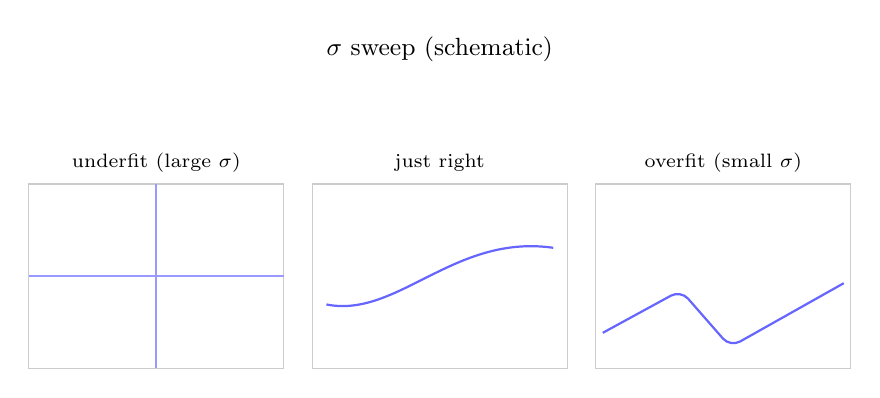
\begin{tikzpicture}[scale=0.9]
        \node at (0,3.2) {\small$\sigma$ sweep (schematic)};
        % three panels
        \begin{scope}[shift={(-4,0)}]
            \draw[gray!40] (-1.8,-1.3) rectangle (1.8,1.3);
            \node at (0,1.6) {\scriptsize underfit (large $\sigma$)};
            \draw[thick, blue!40] (-1.8,0) -- (1.8,0);
            \draw[thick, blue!40] (0,-1.3) -- (0,1.3);
        \end{scope}
        \begin{scope}
            \draw[gray!40] (-1.8,-1.3) rectangle (1.8,1.3);
            \node at (0,1.6) {\scriptsize just right};
            \draw[thick, blue!60, rounded corners] (-1.6,-0.4).. controls (-0.6,-0.6) and (0.2,0.6).. (1.6,0.4);
        \end{scope}
        \begin{scope}[shift={(4,0)}]
            \draw[gray!40] (-1.8,-1.3) rectangle (1.8,1.3);
            \node at (0,1.6) {\scriptsize overfit (small $\sigma$)};
            \draw[thick, blue!60, rounded corners] (-1.7,-0.8) -- (-0.6,-0.2) -- (0.1,-1.0) -- (1.7,-0.1);
        \end{scope}
    \end{tikzpicture}
    % Avoid inline math in captions; it wraps poorly in some EPUB renderers.
\caption{Schematic illustration of how the width parameter \(\sigma\) influences decision boundaries: too-large \(\sigma\) underfits (bases overlap heavily and wash out locality), intermediate \(\sigma\) captures the boundary, and too-small \(\sigma\) can produce fragmented regions. For a computed XOR example, see \Cref{fig:rbf_boundary}.}
    \label{fig:rbf_sigma_sweep}
\end{figure}
\FloatBarrier

We return to this tuning picture again later with an XOR-style toy example, where the decision boundary is easy to visualize.

\paragraph{Notation note.} In this chapter we write radial basis functions as \(\varphi_i(\cdot)\) and use \(\boldsymbol{\Phi}\) for the associated design matrix. When we need a generic kernel feature map, we use \(\phi(\cdot)\) (consistent with \Cref{app:kernels}); when probability density functions are needed, we write them as \(p(\cdot)\). This avoids overloading a single symbol.

% Chapter 8

\subsection{Radial Basis Function Networks: Parameter Estimation and Training}
\label{sec:rbf_radial_basis_function_networks_parameter_estimation_and_training}

Recall that in Radial Basis Function (RBF) networks, the hidden layer neurons compute outputs based on radial basis functions centered at certain points \( \mathbf{v}_i \) with spread parameters \( \sigma_i \). The output is a linear combination of these nonlinear transformations. The key challenge is to determine the parameters:
\[
\{ \mathbf{v}_i, \sigma_i, w_i \}_{i=1}^M,
\]
where \( M \) is the number of hidden neurons.

\paragraph{Finding the Centers \(\mathbf{v}_i\):}
A natural approach to find the centers is to use clustering algorithms on the input data. For example, if we decide to have \( M \) hidden neurons, we run a clustering algorithm (e.g., K-means) to find \( M \) centroids:
\[
\mathbf{v}_1, \mathbf{v}_2, \ldots, \mathbf{v}_M.
\]
These centroids represent typical data points around which the radial basis functions are centered. This approach ensures that the radial basis functions cover the input space effectively.

\paragraph{Determining the Spread Parameters \(\sigma_i\):}
The spread parameters control the width of each radial basis function. One can initialize all \( \sigma_i \) to a common value or assign different values based on the data distribution. A practical rule-of-thumb is
\[
\sigma \approx \frac{d_{\max}}{\sqrt{2M}},
\]
where \(d_{\max}\) is the maximum pairwise distance between centers and \(M\) the number of RBF units; this ensures neighboring receptive fields overlap without collapsing to a constant function. After setting this global width, refine to per-center widths by setting each \( \sigma_i \) proportional to the average distance between the centroid \( \mathbf{v}_i \) and its nearest neighboring centroids. Anisotropic variants scale each dimension separately but follow the same principle of matching the local density of prototypes.

\paragraph{Training the Output Weights \( w_i \):}
Given fixed centers and spreads, the output weights \( w_i \) can be found by minimizing the squared error between the network output and the target values. The network output for an input \( \mathbf{x} \) is:
\[
\hat{y}(\mathbf{x}) = \sum_{i=1}^M w_i \varphi_i(\mathbf{x}).
\]
where
\[
\varphi_i(\mathbf{x}) = \exp\left(-\frac{\|\mathbf{x} - \mathbf{v}_i\|^2}{2\sigma_i^2}\right).
\]

    The training problem reduces to solving the linear system:
\begin{align}
\min_{\mathbf{w}} \| \mathbf{y} - \boldsymbol{\Phi} \mathbf{w} \|^2,
\label{eq:rbf_weight_training}
\end{align}
where \(\mathbf{y}\) is the vector of target outputs and \(\boldsymbol{\Phi}\) is the design matrix with entries \(\boldsymbol{\Phi}_{ji} = \varphi_i(\mathbf{x}_j)\).
When \(\boldsymbol{\Phi}^\top\boldsymbol{\Phi}\) is well-conditioned, the ordinary least-squares solution is
\[
    \mathbf{w}^\star = (\boldsymbol{\Phi}^\top \boldsymbol{\Phi})^{-1}\boldsymbol{\Phi}^\top \mathbf{y}.
\]

\begin{tcolorbox}[summarybox, title={Dual viewpoint: RBFN vs.\ kernel ridge regression}]
Fixing the RBF centers and widths makes the hidden layer a finite basis expansion. Training restricts itself to the \(M\) coefficients \(\mathbf{w}\) and resembles kernel ridge regression with a truncated basis. In the dual view, kernel ridge regression solves
\[
\min_{\boldsymbol{\alpha}} \|\mathbf{y} - \mathbf{K} \boldsymbol{\alpha}\|^2 + \lambda \boldsymbol{\alpha}^\top \mathbf{K} \boldsymbol{\alpha},
\]
where \(\mathbf{K}_{ij} = k(\mathbf{x}_i,\mathbf{x}_j)\) uses the same Gaussian kernel. Setting \(M=N\) and letting the RBF centers coincide with the training points recovers this dual form exactly. Finite \(M\) acts like Nystr\"om approximation: \(\boldsymbol{\Phi} \mathbf{w}\) projects onto a subset of kernel features.

Numerically, \(\boldsymbol{\Phi}^\top \boldsymbol{\Phi}\) can be ill-conditioned if the bases overlap excessively or if centers cluster tightly; kernel ridge has the same issue via \(\mathbf{K}\). Regularization is therefore essential: add \(\lambda I\) before inversion,
\[
\mathbf{w}^\star = (\boldsymbol{\Phi}^\top \boldsymbol{\Phi} + \lambda I)^{-1} \boldsymbol{\Phi}^\top \mathbf{y},
\]
mirroring the \(\lambda \boldsymbol{\alpha}^\top \mathbf{K} \boldsymbol{\alpha}\) term in the dual problem. Larger \(\lambda\) damps coefficients when \(\sigma\) is large (heavy overlap) or when data are noisy, while smaller \(\lambda\) preserves sharper fits at the cost of conditioning. Choosing \(\lambda\) via cross-validation keeps both primal (RBFN) and dual (kernel ridge) systems stable.
\end{tcolorbox}

\Cref{fig:rbf_primal_dual} summarizes the primal and dual viewpoints side by side and highlights where a finite basis acts like a Nystr\"om approximation.

\begin{figure}[t]
    \centering
    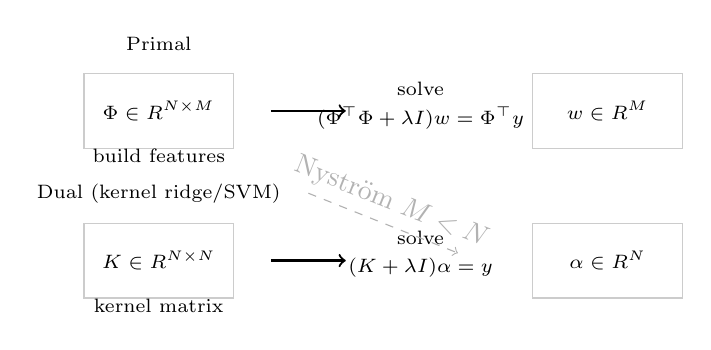
\begin{tikzpicture}[scale=0.95]
        \node at (-3,1.4) {\scriptsize Primal};
        \draw[gray!40] (-4,0) rectangle (-2,1);
        \node[font=\scriptsize] at (-3,0.5) {$\boldsymbol{\Phi}\in\mathbb{R}^{N\times M}$};
        \node[font=\scriptsize] at (-3,-0.1) {build features};
        \draw[->, thick] (-1.5,0.5) -- (-0.5,0.5);
        \node[font=\scriptsize] at (0.5,0.8) {solve};
        \node[font=\scriptsize] at (0.5,0.4) {$(\boldsymbol{\Phi}^\top\boldsymbol{\Phi}+\lambda I)w=\boldsymbol{\Phi}^\top y$};
        \draw[gray!40] (2,0) rectangle (4,1);
        \node[font=\scriptsize] at (3,0.5) {$w\in\mathbb{R}^{M}$};

        \begin{scope}[shift={(0,-2)}]
            \node at (-3,1.4) {\scriptsize Dual (kernel ridge/SVM)};
            \draw[gray!40] (-4,0) rectangle (-2,1);
        \node[font=\scriptsize] at (-3,0.5) {$K\in\mathbb{R}^{N\times N}$};
        \node[font=\scriptsize] at (-3,-0.1) {kernel matrix};
        \draw[->, thick] (-1.5,0.5) -- (-0.5,0.5);
        \node[font=\scriptsize] at (0.5,0.8) {solve};
        \node[font=\scriptsize] at (0.5,0.4) {$(K+\lambda I)\alpha=y$};
        \draw[gray!40] (2,0) rectangle (4,1);
        \node[font=\scriptsize] at (3,0.5) {$\alpha\in\mathbb{R}^{N}$};
    \end{scope}
    \draw[->, gray!60, dashed] (-1,-0.6) -- (1,-1.4) node[midway, sloped, above, gray!60]{Nystr\"om $M<N$};
\end{tikzpicture}
    % Avoid inline math in captions; it wraps poorly in some EPUB renderers.
    \caption{Primal (finite basis) vs.\ dual (kernel ridge) viewpoints. Using as many centers as data points recovers the dual form; using fewer centers corresponds to a Nystr\"om approximation. The same trade-off appears in kernel methods through the choice of kernel and effective rank.}
\label{fig:rbf_primal_dual}
\end{figure}
\FloatBarrier

To improve numerical stability or control model complexity, a Tikhonov (ridge) regulariser can be added,
\[
    \mathbf{w}_\lambda^\star = (\boldsymbol{\Phi}^\top \boldsymbol{\Phi} + \lambda I)^{-1}\boldsymbol{\Phi}^\top \mathbf{y}, \qquad \lambda>0,
\]
or more generally one can use the Moore--Penrose pseudoinverse \(\boldsymbol{\Phi}^{+}\) when \(\boldsymbol{\Phi}^\top\boldsymbol{\Phi}\) is singular, yielding \(\mathbf{w}^\star = \boldsymbol{\Phi}^{+}\mathbf{y}\). A quick dimensional sanity check is that \(\boldsymbol{\Phi}\in\mathbb{R}^{N\times M}\), \(\mathbf{w}\in\mathbb{R}^M\), and \(\mathbf{y}\in\mathbb{R}^N\); all matrix products above respect these shapes.

\paragraph{Iterative Optimization of \(\sigma_i\) and \( w_i \):}
Since both \( \sigma_i \) and \( w_i \) affect the network output, an alternating optimization procedure can be employed:
\begin{enumerate}
    \item Initialize \( \sigma_i \) (e.g., all equal or based on data heuristics).
    \item Fix \( \sigma_i \) and find \( w_i \) by solving the linear least squares problem \eqref{eq:rbf_weight_training}.
    \item Fix \( w_i \) and update \( \sigma_i \) to minimize the error, possibly using gradient-based methods or heuristics.
    \item Repeat steps 2 and 3 until convergence or error criteria are met.
\end{enumerate}

Note that the spreads \( \sigma_i \) can be scalar or vector-valued (anisotropic), allowing different widths in each input dimension:
\[
\sigma_i = [\sigma_{i1}, \sigma_{i2}, \ldots, \sigma_{id}],
\]
where \( d \) is the input dimension.

\paragraph{Summary of the Training Algorithm:}
\begin{enumerate}
    \item Use clustering (e.g., K-means) to find centers \( \mathbf{v}_i \) (or sample centers uniformly at random).
    \item Set widths \(\sigma_i\) via a rule-of-thumb (global \(\sigma\) from average center spacing or per-cluster covariance).
    \item Build \(\boldsymbol{\Phi}\) with entries \(\boldsymbol{\Phi}_{ji}=\varphi_i(\mathbf{x}_j)\); choose a small grid of \(\lambda\) values and solve \((\boldsymbol{\Phi}^\top\boldsymbol{\Phi}+\lambda I)\mathbf{w}=\boldsymbol{\Phi}^\top\mathbf{y}\).
    \item Evaluate on a validation set and pick \((\sigma,\lambda, M)\) that minimizes validation loss; for classification, CE/hinge losses are also feasible with the same design matrix \(\boldsymbol{\Phi}\).
\end{enumerate}

\begin{tcolorbox}[summarybox, title={Practical RBFN training (pseudocode)}]
\begin{verbatim}
Input: X, y, M, center_method=kmeans, sigma_rule, lambda_grid
Centers = center_method(X, M)
sigma = sigma_rule(Centers)
Phi = build_design_matrix(X, Centers, sigma)   # NxM
for lambda in lambda_grid:
    w_lambda = solve((Phi^T Phi + lambda I) w = Phi^T y)
    val_err[lambda] = validation_loss(Phi_val, y_val, w_lambda)
lambda_star = argmin val_err
Predict: yhat(x) = phi(x, Centers, sigma)^T w_lambda_star
\end{verbatim}
\end{tcolorbox}

\paragraph{Worked toy (classification, XOR-like).} Consider four points and XOR labels
\[
\mathbf{x}_1=(0,0),\;\mathbf{x}_2=(0,1),\;\mathbf{x}_3=(1,0),\;\mathbf{x}_4=(1,1),
\qquad \mathbf{t}=[0,1,1,0].
\]
Choose \(M=4\) centers at the data and set a global \(\sigma\) from the mean inter-center distance (here \(\sigma\approx 0.8\)). Build \(\boldsymbol{\Phi}\) with entries \(\boldsymbol{\Phi}_{ji}=\exp\!\big(-\|\mathbf{x}_j-\mathbf{c}_i\|^2/(2\sigma^2)\big)\) and solve \((\boldsymbol{\Phi}^\top\boldsymbol{\Phi}+\lambda I)\mathbf{w}=\boldsymbol{\Phi}^\top\mathbf{t}\) over a small grid \(\lambda\in\{10^{-4},10^{-3},10^{-2}\}\). The best \(\lambda\) yields a linear separator in the lifted \(\boldsymbol{\Phi}\)-space that classifies XOR. Widening \(\sigma\) makes bases overlap heavily and can wash out locality (very smooth boundaries and low margins), while shrinking \(\sigma\) makes the model extremely local and can create small islands that fit the training points but generalize poorly. Ridge helps whenever \(\boldsymbol{\Phi}^\top\boldsymbol{\Phi}\) is poorly conditioned (typically when bases overlap heavily or centers cluster).

\Cref{fig:rbf_boundary} shows one such boundary for a fixed choice of centers, width, and ridge regularization.

	    \begin{figure}[t]
	        \centering
	            % Reproduce the plots directly in PGFPlots so they remain grayscale/KDP-safe.
	            % Data tables are generated by `notes_output/scripts/gen_rbf_xor_sigma_sweep_tables.py`.
	            \begin{tikzpicture}
	            \pgfplotsset{colormap={rbfclass}{
	                % Light vs. darker tint: still distinct in grayscale, but more pleasant in color.
	                color(0cm)=(white);
	                color(1cm)=(cbBlue!35)
	            }}
                \begin{groupplot}[
                    group style={group size=3 by 1, horizontal sep=0.9cm},
                    width=0.31\linewidth,
                    height=0.31\linewidth,
                    xmin=-0.2, xmax=1.2,
                    ymin=-0.2, ymax=1.2,
                    grid=both,
                    grid style={gray!10},
                    axis on top,
                    clip=false,
                    colormap name=rbfclass,
                    point meta min=0,
                    point meta max=1,
                    xlabel={$x_1$},
                    xtick={0,1},
                    ytick={0,1},
                    tick label style={font=\scriptsize},
                    label style={font=\scriptsize},
                    title style={font=\scriptsize, align=center},
                ]
                \nextgroupplot[title={$\sigma=2.0$ (too broad)}, ylabel={$x_2$}]
                    \addplot[
                        matrix plot*,
                        mesh/cols=29,
                        mesh/rows=29,
                        point meta=explicit,
                        forget plot,
                    ] table [x=x, y=y, meta=cls] {rbf_xor_sigma2p0_boundary_class_table_with_breaks.dat};
                    \addplot[
                        black,
                        very thick,
                        unbounded coords=jump,
                        forget plot,
                    ] table [x=x, y=y] {rbf_xor_sigma2p0_contour_0p5.dat};
                    \addplot[only marks, mark=o, mark options={fill=white, draw=black}, mark size=2.6pt, forget plot]
                        coordinates {(0,0) (1,1)};
                    \addplot[only marks, mark=square*, mark options={fill=black, draw=black}, mark size=2.6pt, forget plot]
                        coordinates {(0,1) (1,0)};

                \nextgroupplot[title={$\sigma=0.8$ (balanced)}]
                    \addplot[
                        matrix plot*,
                        mesh/cols=29,
                        mesh/rows=29,
                        point meta=explicit,
                        forget plot,
                    ] table [x=x, y=y, meta=cls] {rbf_xor_sigma0p8_boundary_class_table_with_breaks.dat};
                    \addplot[
                        black,
                        very thick,
                        unbounded coords=jump,
                        forget plot,
                    ] table [x=x, y=y] {rbf_xor_sigma0p8_contour_0p5.dat};
                    \addplot[only marks, mark=o, mark options={fill=white, draw=black}, mark size=2.6pt, forget plot]
                        coordinates {(0,0) (1,1)};
                    \addplot[only marks, mark=square*, mark options={fill=black, draw=black}, mark size=2.6pt, forget plot]
                        coordinates {(0,1) (1,0)};

                \nextgroupplot[title={$\sigma=0.25$ (too local)}]
                    \addplot[
                        matrix plot*,
                        mesh/cols=29,
                        mesh/rows=29,
                        point meta=explicit,
                        forget plot,
                    ] table [x=x, y=y, meta=cls] {rbf_xor_sigma0p25_boundary_class_table_with_breaks.dat};
                    \addplot[
                        black,
                        very thick,
                        unbounded coords=jump,
                        forget plot,
                    ] table [x=x, y=y] {rbf_xor_sigma0p25_contour_0p5.dat};
                    \addplot[only marks, mark=o, mark options={fill=white, draw=black}, mark size=2.6pt, forget plot]
                        coordinates {(0,0) (1,1)};
                    \addplot[only marks, mark=square*, mark options={fill=black, draw=black}, mark size=2.6pt, forget plot]
                        coordinates {(0,1) (1,0)};
                \end{groupplot}
	        \end{tikzpicture}
	        % Avoid inline math in captions; it wraps poorly in some EPUB renderers.
	        \caption{Effect of \(\sigma\) on an RBFN XOR boundary (4 centers at the data corners, ridge \(\lambda=10^{-3}\), threshold 0.5). Too-large \(\sigma\) makes bases overlap heavily, producing a very smooth, low-contrast boundary; intermediate \(\sigma\) yields a cleaner separation; too-small \(\sigma\) makes the model extremely local, producing small ``islands'' around prototypes.}
	        \label{fig:rbf_boundary}
	    \end{figure}
\FloatBarrier


\subsection{Remarks on Radial Basis Function Networks}
\label{sec:rbf_remarks_on_radial_basis_function_networks}

\paragraph{Advantages:}
\begin{itemize}
    \item \textbf{Training speed:} Once centers and spreads are fixed, training reduces to a linear least squares problem with a closed-form solution, which is computationally efficient.
    \item \textbf{Universal approximation:} RBF networks can approximate any continuous function on a compact domain to arbitrary accuracy given sufficient neurons, provided the centers cover the domain and the widths are chosen to avoid degeneracy \citep{Micchelli1986,ParkSandberg1991}.
    \item \textbf{Interpretability:} Centers correspond to representative data points, making the network structure more interpretable.
    \item \textbf{Applications:} RBF networks have been successfully applied in control systems, communication systems, chaotic time series prediction (e.g., weather and power load forecasting), and decision-making tasks.
    \item \textbf{Flexible losses:} Squared loss is standard for regression; logistic or hinge losses pair naturally with the fixed design matrix for classification.
\end{itemize}

\paragraph{Disadvantages:}
\begin{itemize}
    \item \textbf{Parameter selection:} Choosing the number of neurons \( M \), centers \( \mathbf{v}_i \), and spreads \( \sigma_i \) is nontrivial and often requires heuristics or cross-validation.
    \item \textbf{Scalability:} The number of radial units required can grow quickly with input dimensionality, increasing computation and storage costs.
    \item \textbf{Center determination:} Identifying good centers (via clustering or other heuristics) can be computationally expensive and sensitive to noisy data.
\end{itemize}

% Chapter 8: Finalizing Derivations and Closure

\begin{tcolorbox}[summarybox, title={Sidebar (optional): Wiener filtering in one paragraph}]
The Wiener filter is the same least-squares projection story in signal-processing notation. In the Wiener case, you write the linear estimator as \(y(t)=\mathbf{w}^\top\mathbf{x}(t)\) and the normal equations involve second-order statistics \(\mathbf{R}=\mathbb{E}[\mathbf{x}\mathbf{x}^\top]\) and \(\mathbf{p}=\mathbb{E}[d\,\mathbf{x}]\), giving \(\mathbf{R}\mathbf{w}^\star=\mathbf{p}\). In an RBF network, you replace the raw input \(\mathbf{x}\) by fixed nonlinear features \(\boldsymbol{\Phi}\) (built from radial units), and the same idea becomes \((\boldsymbol{\Phi}^\top\boldsymbol{\Phi}+\lambda I)\mathbf{w}^\star=\boldsymbol{\Phi}^\top\mathbf{y}\). The point of the sidebar is just this mapping: both are ``fit a linear readout to fixed features,'' and conditioning/regularization control how stable that fit is.
\end{tcolorbox}

\subsection{Preview: Unsupervised and Localized Learning}
\label{sec:rbf_preview_unsupervised_and_localized_learning}

In \Cref{chap:som}, we move from supervised RBF models to unsupervised, self-organizing methods. Self-organizing maps (SOMs) and Hopfield-style associative memory discover structure in data (clusters, manifolds) without labeled targets, complementing the supervised architectures covered so far.

\begin{tcolorbox}[summarybox, title={Key takeaways}]
\textbf{Minimum viable mastery}
\begin{itemize}
    \item Localized Gaussian bases + linear readout give an interpretable nonlinear model; center/width/regularization choices control bias--variance.
    \item Primal RBFNs and kernel ridge regression are two views of the same estimator (full vs. truncated basis); regularization cures conditioning.
    \item RBFNs bridge learned-feature models (MLPs) and kernel methods (SVMs/GPs); they form a strong baseline for localized decision boundaries.
\end{itemize}
\medskip
\textbf{Common pitfalls}
\begin{itemize}
    \item Width selection: too small memorizes, too large collapses to a linear model; validate \(\sigma\) and \(\lambda\).
    \item Poor conditioning: without regularization, solves can be numerically unstable even when the math is correct.
    \item Confusing kernels with bases: a full kernel method scales differently than a truncated (primal) basis expansion.
\end{itemize}
\end{tcolorbox}

\begin{tcolorbox}[summarybox, title={Exercises and lab ideas}]
\begin{itemize}
    \item Train an RBFN on the two-moons dataset; sweep \(M\) and \(\sigma\), add a small \(\lambda\) grid, plot validation curves and decision boundaries; report the \((M,\sigma,\lambda)\) that minimizes validation error and discuss over/underfitting.
    \item Compare primal RBFN and kernel ridge regression with an RBF kernel on datasets of size \(N\in\{200,2000,20\,000\}\); measure accuracy and runtime; note when each approach is preferable.
    \item Show that setting centers at all data points with \(\lambda>0\) yields the same predictions as kernel ridge regression; derive the relationship between \(\mathbf{w}\) and \(\boldsymbol{\alpha}\).
    \item Plot how validation error moves with \((M,\sigma,\lambda)\) and link the curves back to the bias--variance discussion in \Cref{chap:supervised}.
\end{itemize}
\medskip
\noindent\textbf{If you are skipping ahead.} Keep the idea that ``nonlinear'' can still be linear-in-parameters once a basis is fixed. That perspective is reused in kernel methods and shows up again when we discuss architectural bias (CNNs) and representation choices.
\end{tcolorbox}

\medskip
\paragraph{Where we head next.} \Cref{chap:som} moves from supervised objectives to unlabeled competitive learning and prototype organization. \Cref{chap:hopfield} then revisits recurrence through an energy-based lens, setting up later sequence-model chapters.

\nocite{Haykin2013AdaptiveFilterTheory, WidrowStearns1985, SchreierScharf2010, Micchelli1986, ParkSandberg1991, PoggioGirosi1990, Bishop1995, HastieTibshiraniFriedman2009}
